% ============================================================================
% CHAPITRE 2 — ÉTAT DE L'ART ET FONDEMENTS THÉORIQUES (Part 1: 2.1–2.3)
% ============================================================================

\section{Introduction}

Ce chapitre établit les fondements théoriques et bibliographiques sur lesquels repose la
conception du système Guidni. Il couvre cinq domaines majeurs~: les agents conversationnels
basés sur les grands modèles de langage (LLM), la génération augmentée par récupération (RAG),
les systèmes de recommandation classiques, les bandits multi-bras contextuels et en particulier
l'algorithme Thompson Sampling Hybride, ainsi qu'une revue comparative des travaux connexes. Pour chaque domaine,
la présentation progresse des concepts généraux vers les choix spécifiques retenus pour le
projet Guidni.

L'objectif de ce chapitre est double~: d'une part, fournir au lecteur les clés de compréhension
nécessaires pour appréhender les décisions architecturales présentées dans les chapitres suivants~;
d'autre part, situer la contribution de ce projet par rapport à l'état actuel de la recherche et
des systèmes industriels dans les domaines de la planification touristique intelligente et de la
recommandation personnalisée en temps réel.


% ────────────────────────────────────────────────────────────────
\section{Agents LLM et planification conversationnelle}
% ────────────────────────────────────────────────────────────────

\subsection{Les grands modèles de langage (LLMs)}

L'architecture Transformer, introduite par Vaswani et al. en 2017~\cite{vaswani2017attention},
constitue le socle de tous les grands modèles de langage modernes. Son innovation centrale réside
dans le mécanisme d'attention multi-têtes (\textit{multi-head attention}), qui permet au modèle
de pondérer l'importance relative de chaque token d'entrée par rapport à tous les autres, quelle
que soit leur distance dans la séquence. Contrairement aux architectures récurrentes qui traitent
les tokens séquentiellement, le Transformer traite l'ensemble de la séquence en parallèle, ce qui
permet un entraînement massivement distribué sur des corpus de texte de plusieurs téraoctets.

L'évolution des LLMs a connu une étape décisive avec l'introduction de l'ajustement par
instructions (\textit{instruction tuning}) et de l'apprentissage par renforcement à partir de
retours humains (RLHF --- \textit{Reinforcement Learning from Human Feedback}). Ces techniques
transforment un modèle de prédiction de tokens en un assistant capable de comprendre et d'exécuter
des instructions formulées en langage naturel. Le modèle n'apprend plus seulement à compléter
une séquence statistiquement probable, mais à produire des réponses utiles, structurées et
conformes aux attentes de l'utilisateur.

L'émergence de l'appel d'outils (\textit{tool use} ou \textit{function calling}) constitue une
avancée fondamentale pour la construction d'agents autonomes. Dans ce paradigme, le LLM n'essaie
pas de générer la réponse directement depuis sa mémoire paramétrique~; il émet plutôt un objet
JSON structuré décrivant quelle fonction externe appeler et avec quels arguments. Par exemple,
au lieu d'inventer les conditions météorologiques à Djerba, le modèle peut appeler explicitement
\texttt{get\_weather(location="Djerba", date="2026-01-15")} et recevoir en retour des données
réelles de l'API Open-Meteo.

Cette capacité d'appel d'outils est fondamentale pour la construction d'agents fiables qui
accèdent à des données en temps réel, des bases de données et des APIs externes. Un LLM sans
outils est contraint de répondre uniquement à partir de ses données d'entraînement, ce qui
entraîne inévitablement des hallucinations factuelles~--- des informations plausibles mais
fausses. Pour un planificateur de voyage, ce problème est particulièrement critique~: recommander
un hôtel inexistant, un prix erroné ou une activité fermée détruit immédiatement la confiance de
l'utilisateur. L'accès aux outils transforme le LLM d'un générateur de texte en un orchestrateur
de données vérifiées.

\begin{figure}[H]
    \centering
    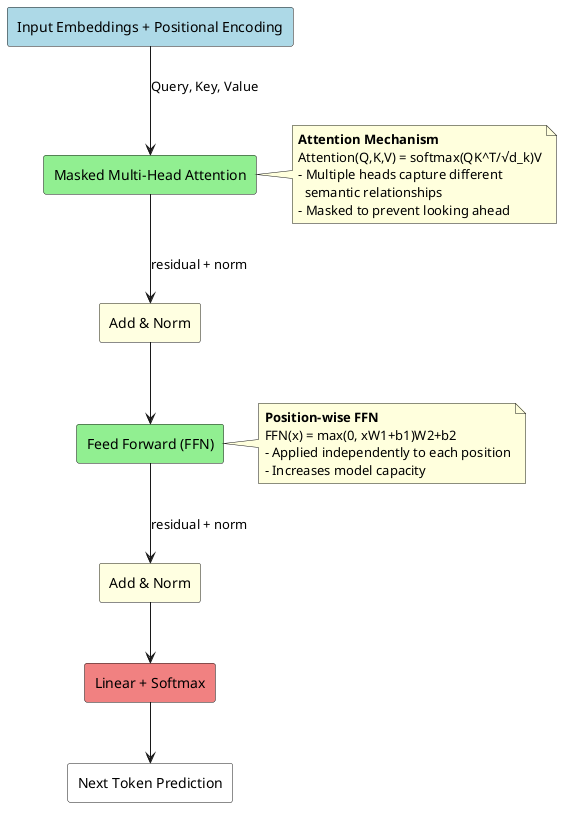
\includegraphics[width=\textwidth]{diagrams/fig_02_transformer_attention.png}
    \caption{Architecture simplifiée d'un décodeur Transformer avec mécanisme d'attention}
    \label{fig:transformer}
\end{figure}


\subsection{Frameworks agentiques~: ReAct et LangGraph}

Le patron ReAct (\textit{Reason + Act}), proposé par Yao et al.~\cite{yao2023react}, formalise
le cycle de raisonnement agentique~: à chaque étape, le modèle raisonne sur la situation courante,
décide d'une action à entreprendre (typiquement un appel d'outil), observe le résultat retourné,
puis raisonne à nouveau sur la base de cette nouvelle information. Ce cycle simple mais puissant
permet de résoudre des tâches complexes en plusieurs étapes, où chaque étape affine la
compréhension du problème et rapproche l'agent de la solution finale.

Toutefois, une boucle ReAct simple ne suffit pas pour une tâche aussi structurée que la
planification de voyage. Un cycle réflexion-action sans contrainte ne dispose d'aucun mécanisme
pour vérifier la cohérence d'un plan généré, ne peut empêcher l'agent de tourner indéfiniment
lorsque le raisonnement devient circulaire, et ne prévoit pas la transmission progressive des
étapes intermédiaires à l'interface utilisateur. Ces limitations appellent un cadre plus
expressif, capable de modéliser explicitement les états de l'agent et les transitions autorisées.

LangGraph, développé par LangChain Inc., étend le concept ReAct avec une machine à états typée
explicite. L'état de l'agent est défini par un \texttt{TypedDict} Python appelé \texttt{AgentState}
qui accumule les messages via l'opérateur \texttt{operator.add}, et suit l'ensemble des données
collectées~: profil utilisateur, activités trouvées, météo, hébergements, restaurants, contexte
RAG, plan en cours de construction, étapes de raisonnement, outils utilisés, compteur d'itérations,
et indicateurs de décision (besoin d'information supplémentaire, plan prêt pour validation). Des
fonctions de routage conditionnel déterminent quel nœud s'exécute ensuite en fonction de l'état
courant, et le mode streaming permet l'affichage en temps réel des étapes de réflexion dans
l'interface utilisateur.

Le graphe spécifique construit pour l'agent Guidni comporte quatre nœuds~: \textbf{THINK}
(le LLM analyse la situation et décide de l'action suivante), \textbf{EXECUTE\_TOOL} (l'outil
appelé s'exécute et retourne un résultat), \textbf{VALIDATE} (vérification de la cohérence
d'un plan généré), et \textbf{RESPOND} (formulation de la réponse finale). La topologie du
graphe est la suivante~: le point d'entrée est THINK~; après réflexion, un routage conditionnel
oriente l'exécution vers l'appel d'outil si le LLM a émis une requête instrumentale, vers la
validation si un plan structuré est prêt, vers la réponse si l'agent a besoin d'informations
supplémentaires de l'utilisateur, ou vers une sortie forcée si le nombre maximal d'itérations
est atteint. Après l'exécution d'un outil, l'agent retourne à la phase de réflexion pour
réévaluation, sauf lorsqu'une question est adressée à l'utilisateur, auquel cas la réponse est
transmise directement. Après la validation, l'agent revient à la phase de réflexion si des
erreurs ont été détectées et qu'il reste des itérations, ou formule la réponse finale si la
validation a réussi.

LangGraph a été préféré aux alternatives plus simples (chaînes LangChain Expression Language,
CrewAI) pour plusieurs raisons~: l'état explicite facilite le débogage en rendant visible
l'ensemble des données accumulées à chaque étape, la boucle de validation garantit la cohérence
des plans générés avant leur présentation à l'utilisateur, la sortie forcée à 15~itérations
empêche les boucles infinies en cas de raisonnement circulaire, et le support du streaming
permet d'afficher les étapes de réflexion (\textit{thinking steps}) de manière progressive dans
l'interface frontend, offrant une expérience utilisateur transparente.

% --- PlantUML diagram placeholder ---
\begin{figure}[H]
    \centering
    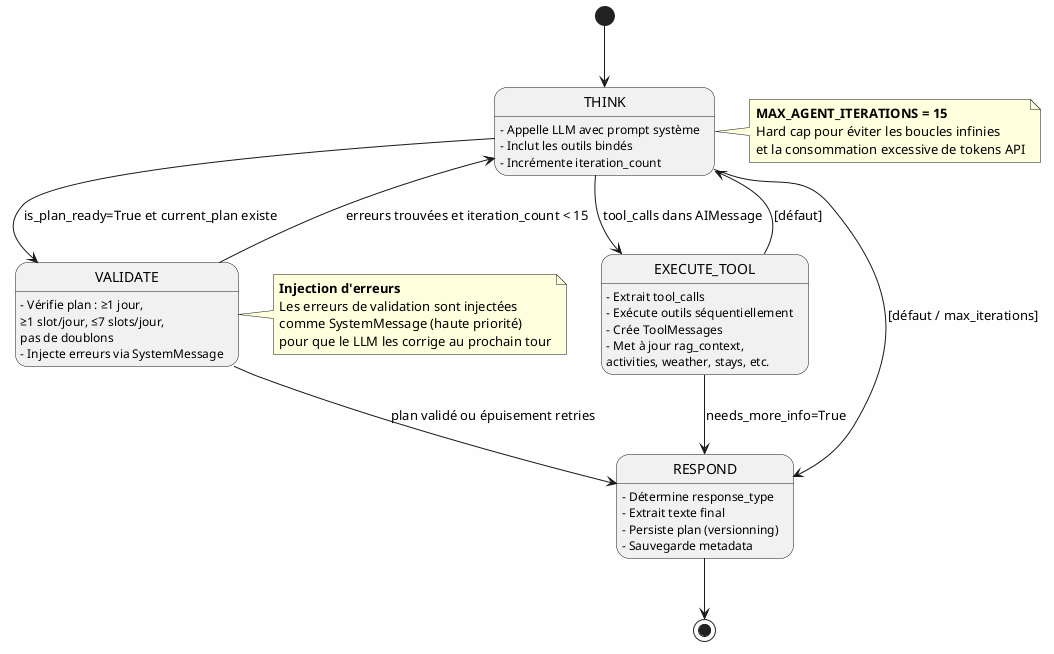
\includegraphics[width=\textwidth]{diagrams/fig_02_langgraph_graph.png}
    \caption{Graphe LangGraph de l'agent planificateur Guidni}
    \label{fig:langgraph}
\end{figure}

% --- Sequence diagram placeholder ---
\begin{figure}[H]
    \centering
    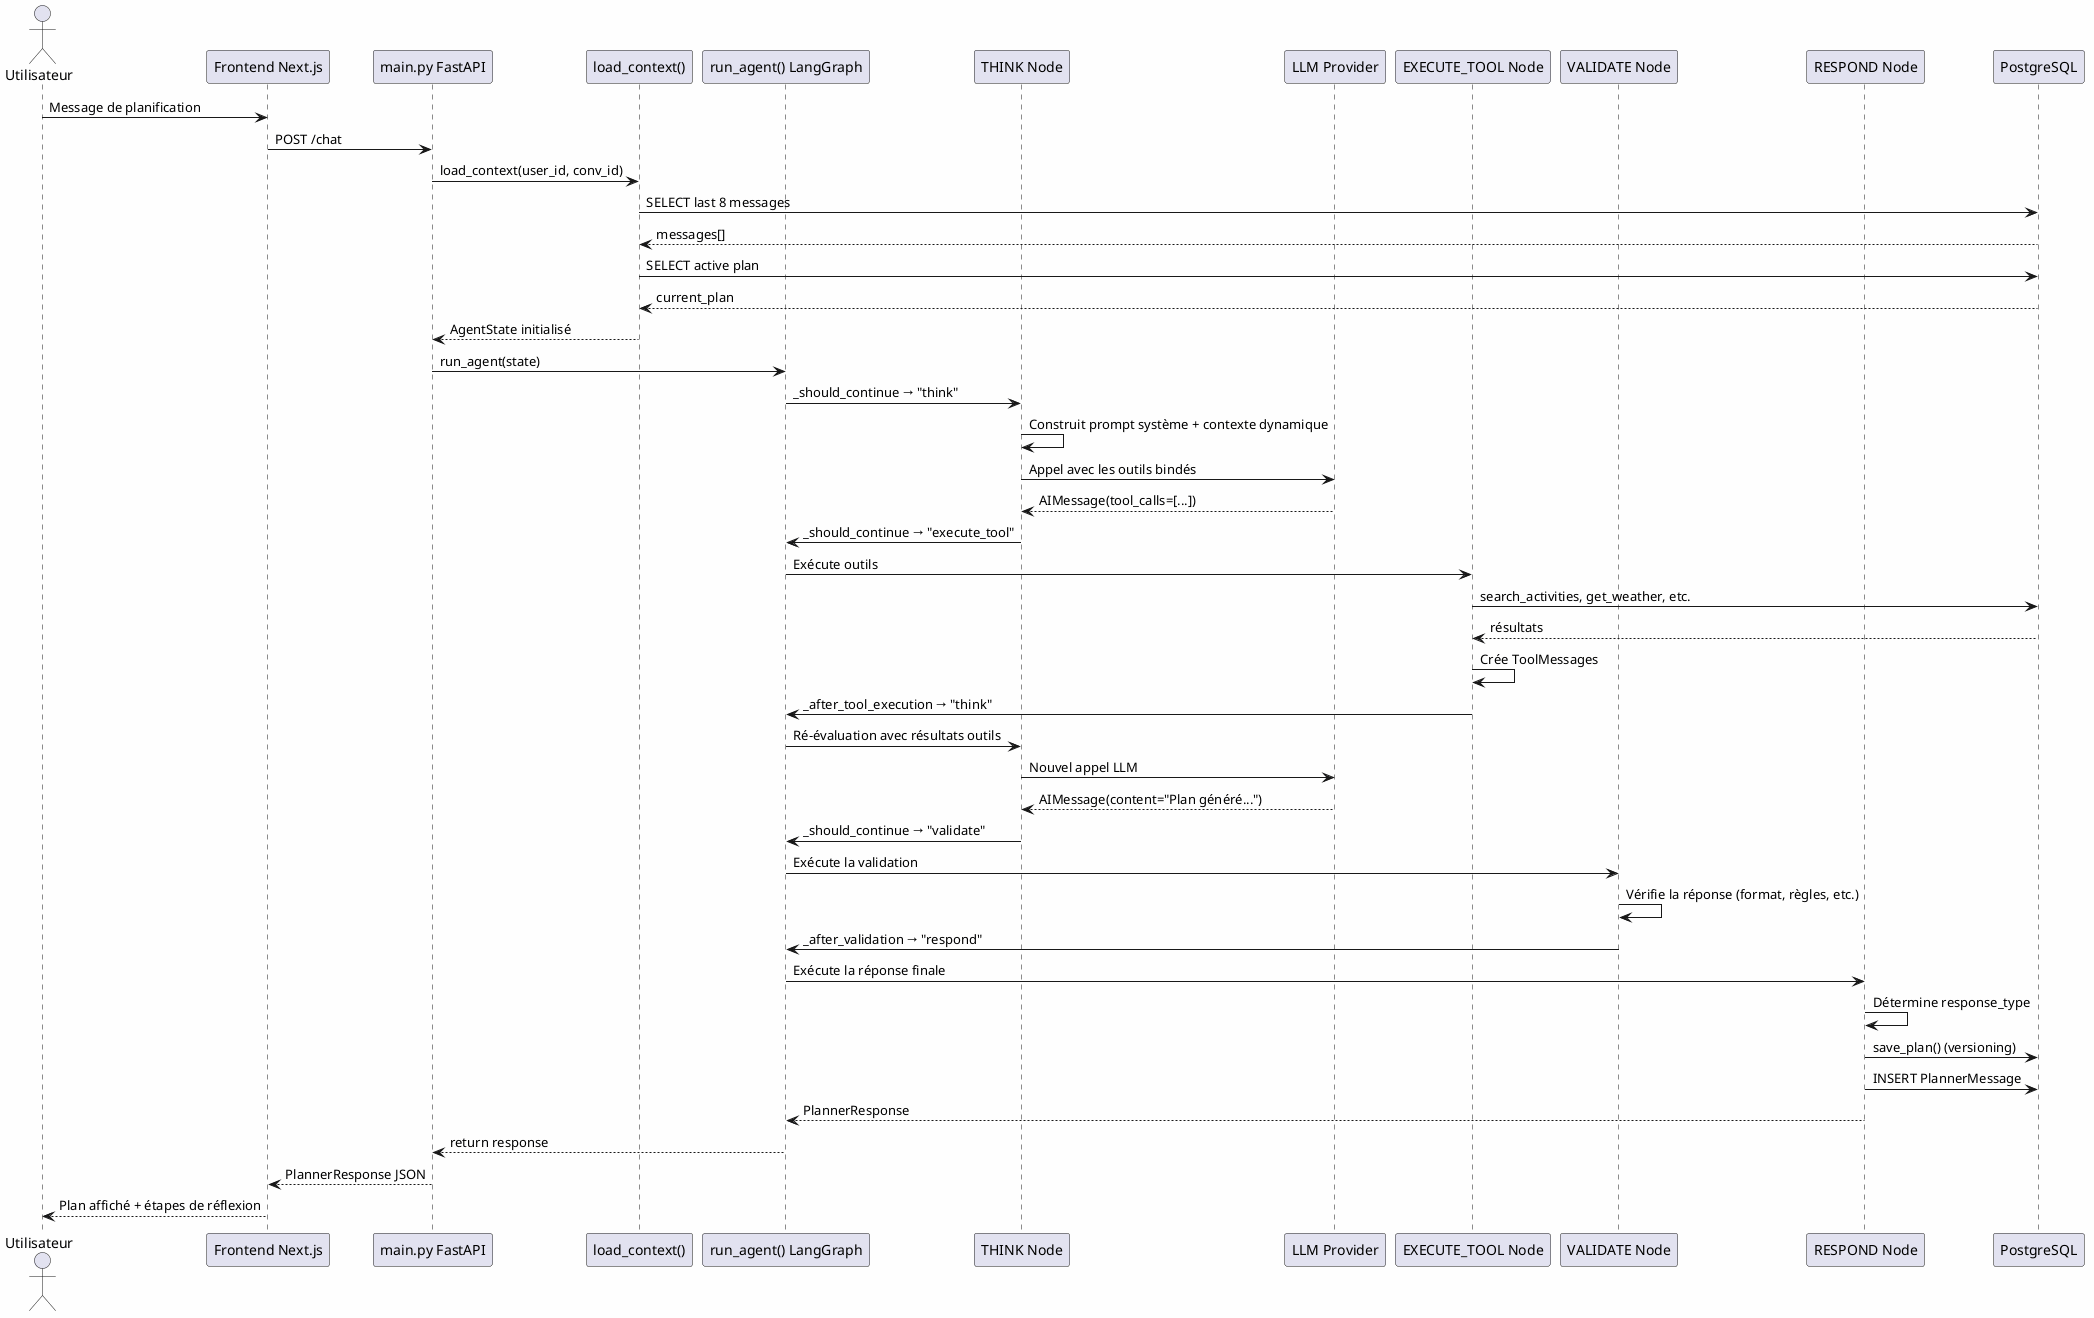
\includegraphics[width=\textwidth]{diagrams/fig_02_agent_sequence.png}
    \caption{Diagramme de séquence d'un cycle complet de l'agent}
    \label{fig:agent_sequence}
\end{figure}


\subsection{Abstraction multi-fournisseurs LLM}

L'abstraction de l'accès aux fournisseurs LLM constitue un choix architectural essentiel pour
tout système agentique destiné à un usage en production. Les coûts varient considérablement
d'un fournisseur à l'autre~--- Ollama est gratuit mais plus lent car il s'exécute localement,
Groq offre une inférence ultra-rapide mais impose des quotas d'utilisation, Gemini propose la
fenêtre de contexte la plus large (jusqu'à un million de tokens) mais engendre des coûts API.
La latence diffère un modèle local à 7~milliards de paramètres et un
modèle cloud optimisé. De plus, certains environnements de déploiement exigent un fonctionnement
entièrement hors ligne, rendant indispensable la possibilité de basculer entre fournisseurs sans
modification du code applicatif.

Dans le contexte d'un projet académique, cette capacité de commutation revêt une importance
particulièrement concrète~: le développeur doit pouvoir itérer hors ligne avec un modèle local
gratuit lors des phases de prototypage, puis basculer vers un modèle cloud performant pour
l'évaluation qualitative, sans modifier une seule ligne du code agentique. Il ne s'agit donc
pas d'une préférence théorique mais d'une exigence d'ingénierie opérationnelle.

Le système Guidni implémente un patron fabrique (\textit{factory pattern}) qui route les
requêtes vers le fournisseur approprié sur la base d'une simple chaîne de configuration,
maintenant le code agentique entièrement découplé des implémentations spécifiques à chaque
fournisseur.

Le système supporte en outre la sélection du modèle au niveau de chaque requête individuelle,
permettant une commutation dynamique sans redémarrage du serveur. Cette flexibilité offre aux
utilisateurs avancés la possibilité de comparer les performances de différents modèles sur une
même requête de planification.

\begin{table}[H]
    \centering
    \caption{Comparaison des fournisseurs LLM intégrés dans Guidni}
    \label{tab:llm_providers}
    \small
    \begin{tabular}{p{1.8cm} p{2.8cm} p{1.2cm} p{1.5cm}  p{2.5cm} p{2.5cm}}
        \toprule
        \textbf{Fournisseur} & \textbf{Modèle} & \textbf{Type} & \textbf{Contexte} &
        \textbf{Points forts} & \textbf{Contraintes} \\
        \midrule
        Ollama & qwen2.5:7b & Local & 8\,192 tok. & 
        Gratuit, confidentialité, hors-ligne & Lent, RAM requise \\[4pt]
        Groq & llama-3.3-70b-versatile & Cloud & 12k tok. & 
        Très rapide, essai gratuit & Quota API, réseau \\[4pt]
        Gemini & gemini-2.5-flash & Cloud & 1M tok. &
        Multimodal, contexte énorme & Coût API\\[4pt]
        Lightning & openai/gpt-5 & Cloud & 400k tok. &Dernière génération & Réseau, coût \\
        \bottomrule
    \end{tabular}
\end{table}

La section suivante aborde le mécanisme de génération augmentée par récupération (RAG), qui
permet à l'agent d'accéder à des données locales vérifiées plutôt que de s'appuyer sur la mémoire
paramétrique du LLM.


% ────────────────────────────────────────────────────────────────
\section{Génération augmentée par récupération (RAG)}
% ────────────────────────────────────────────────────────────────

\subsection{Motivation et principe}

Le problème fondamental que résout la technique RAG est l'incapacité des LLMs à connaître des
informations spécifiques à un domaine local. Les modèles de langage sont entraînés sur des corpus
internet généraux et ne peuvent pas connaître les caractéristiques précises d'un hôtel à Djerba,
le menu d'un restaurant local, ou le prix actuel d'une activité de plongée. Interroger un LLM sur
\og{}l'Hôtel Djerba Plaza\fg{} ou \og{}le Restaurant Haroun\fg{} sans contexte produira des
descriptions hallucinées~--- des informations plausibles mais factuellement fausses. Pour un
planificateur de voyage, cette situation est catastrophique car les utilisateurs font confiance
aux adresses, prix et horaires recommandés.

Le principe RAG (\textit{Retrieval-Augmented Generation}), formalisé par Lewis et al.~\cite{lewis2020rag},
repose sur une idée simple mais efficace~: au lieu de s'appuyer sur la mémoire paramétrique du LLM,
le système récupère des documents pertinents depuis une base de connaissances structurée et les
injecte comme contexte dans le prompt. Le LLM raisonne alors sur des données réelles et vérifiées
plutôt que d'inventer des informations. Cette approche combine la capacité de raisonnement et de
génération fluide du LLM avec la précision factuelle d'une base de données interrogée en temps réel.

L'architecture RAG se décompose en deux phases distinctes. La \textbf{phase d'indexation}, exécutée
au démarrage de l'application, convertit l'ensemble des enregistrements de la base de données en
documents textuels, calcule les vecteurs d'embedding pour chaque document, et construit un index
vectoriel interrogeable. La \textbf{phase de requête}, exécutée à chaque demande utilisateur,
prend la requête en entrée, trouve les documents sémantiquement similaires dans l'index, et
retourne les résultats les plus pertinents avec leurs scores de similarité.

L'implémentation Guidni indexe six types d'entités~: les activités (\texttt{Activity}), les
hébergements (\texttt{Stay}), les restaurants (\texttt{Restaurant}), les attractions
(\texttt{Attraction}), les locations (\texttt{Rental}) et les transferts (\texttt{Transfer}).
Chaque entité est convertie en un document textuel riche englobant ses informations textuelles 
principales (comme le titre et la description complète). Ce document est accompagné d'un 
dictionnaire de métadonnées structurées, utilisé pour le filtrage précis lors des requêtes. 
Afin d'optimiser le système, ce schéma de métadonnées est dynamique~: il combine des champs 
de base communs à toutes les entités (type d'entité, identifiant, destination, prix) avec 
des attributs spécifiques injectés selon la nature de l'entité (ex.~: \texttt{tags} pour les 
équipements d'un hôtel, ou \texttt{capacity} pour un véhicule de location).

\texttt{VECTOR\_ENGINE}.

% --- RAG architecture diagram ---
\begin{figure}[H]
    \centering
    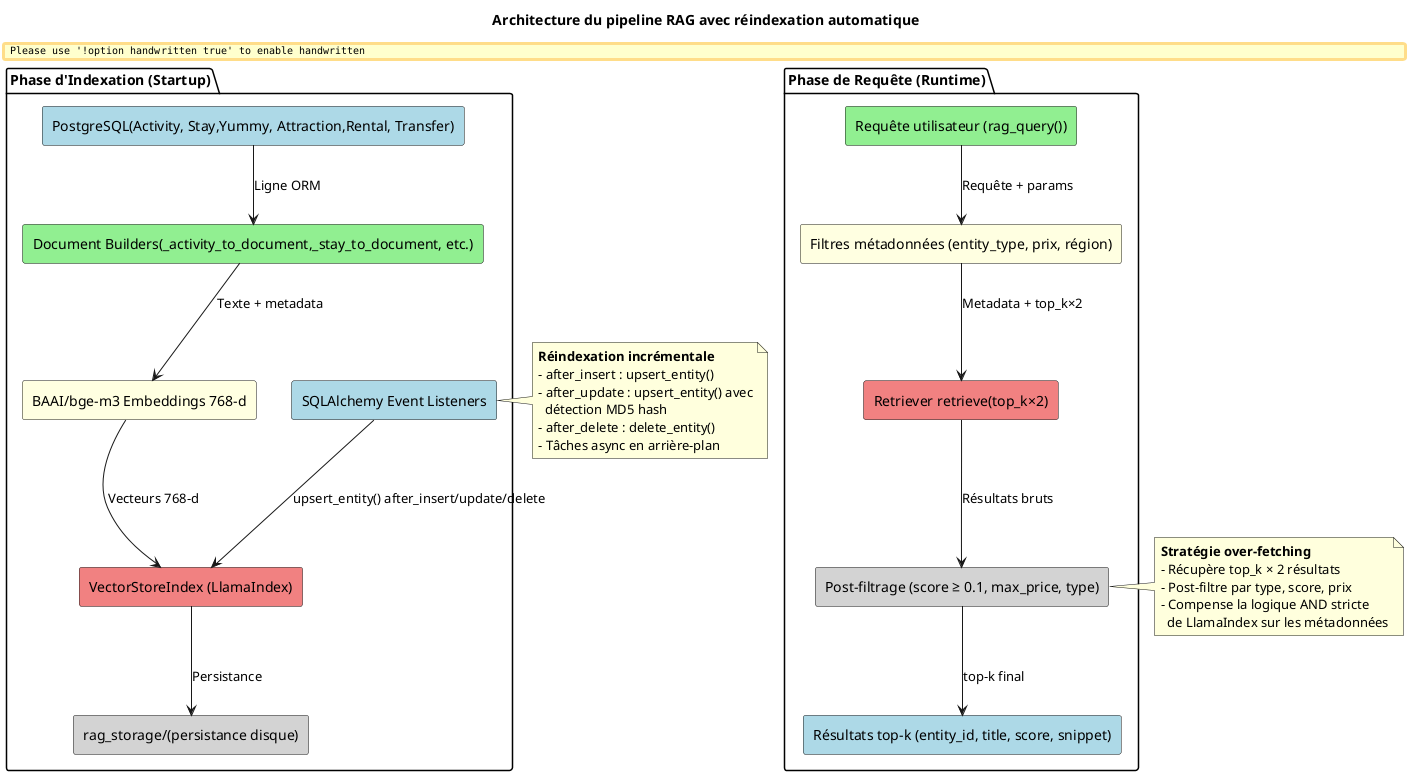
\includegraphics[width=\textwidth]{diagrams/fig_02_rag_architecture.png}
    \caption{Architecture du pipeline RAG avec réindexation automatique}
    \label{fig:rag_architecture}
\end{figure}


\subsection{Modèle d'embedding BAAI/bge-m3}

Le modèle BAAI/bge-m3, publié par la Beijing Academy of Artificial Intelligence, est un modèle
d'embedding multilingue open source supportant plus de 100~langues, dont le français, l'anglais
et l'arabe. Il produit des vecteurs denses de 1024~dimensions qui capturent la signification
sémantique des textes indépendamment de la langue~: une requête en français sur \og{}plage
familiale\fg{} retrouvera des documents mentionnant \og{}family beach\fg{} en anglais ou
des termes équivalents en arabe. Cette propriété multilingue est
essentielle pour le marché touristique de Djerba, intrinsèquement trilingue.

Le modèle est exécuté localement sur CPU avec des paramètres de découpage standard, ne
nécessitant ni GPU ni appel à une API externe.

Le choix de bge-m3 par rapport aux alternatives a été motivé par plusieurs facteurs~: il est
gratuit (aucune clé API nécessaire), respectueux de la vie privée (exécution entièrement locale),
multilingue de manière native --- ce qui est critique pour le marché touristique FR/EN/AR --- et
surpasse les modèles plus petits sur les benchmarks de récupération pour du contenu multi-domaine.
L'alternative OpenAI \texttt{text-embedding-3} offre des performances similaires mais introduit
une dépendance réseau, un coût par requête et une transmission des données hors du serveur.

\subsection{Ré-ordonnancement par Cross-Encoder}

Pour pallier les limites de la recherche vectorielle classique (Bi-Encoder), le système intègre une approche 
de recherche en deux étapes (\textit{two-stage retrieval}). Après une première récupération large, un modèle 
Cross-Encoder (\texttt{BAAI/bge-reranker-v2-m3}) évalue conjointement la requête de l'utilisateur et chaque 
document candidat. Cette méthode permet de capturer des nuances sémantiques complexes et d'attribuer un score 
de pertinence d'une grande précision avant l'injection dans le prompt du LLM.

\subsection{Réindexation automatique via Triggers SQL}

Le problème résolu par la réindexation automatique est le suivant~: si un propriétaire d'hôtel 
met à jour le prix de son annonce ou si une nouvelle activité est ajoutée à la base de données, 
l'index vectoriel devient obsolète et l'agent recommandera des informations périmées. Une reconstruction 
manuelle de l'index nécessiterait une intervention technique lourde, ce qui est inacceptable pour un système en production.

La solution retenue repose sur la mise en place de déclencheurs (triggers) directement au niveau 
de la base de données. Des triggers sont attachés aux opérations d'insertion, de mise à jour et de suppression 
sur les tables correspondant aux six types d'entités couverts par la plateforme. Lorsqu'une modification survient 
au niveau des données, la base de données capture nativement l'événement et notifie le système pour déclencher une 
tâche asynchrone en arrière-plan. Cette tâche se charge alors de recalculer l'embedding de manière isolée pour l'entité concernée.

Les bénéfices de cette approche sont multiples~: l'index reste toujours 
à jour sans aucune intervention manuelle et le système gagne en robustesse. En effet, en opérant au niveau 
de la base de données, les modifications sont détectées même si elles sont effectuées en dehors de l'application 
principale (indépendance vis-à-vis de l'ORM). De plus, la réindexation est non bloquante car elle s'exécute en 
arrière-plan via des tâches asynchrones, et le traitement est ciblé --- seule l'entité modifiée est réindexée, 
et non l'ensemble du corpus. Cette architecture garantit que l'agent planificateur travaille systématiquement sur 
des données actualisées.

La section suivante élargit la perspective aux systèmes de recommandation, domaine théorique qui sous-tend 
le second sous-système du projet Guidni.
% ============================================================================
% CHAPITRE 2 — ÉTAT DE L'ART (Part 2: 2.4–2.6 + Conclusion)
% ============================================================================

% ────────────────────────────────────────────────────────────────

\section{Systèmes de recommandation~: vue d'ensemble}
% ────────────────────────────────────────────────────────────────

Le \textbf{filtrage collaboratif} repose sur la matrice d'interactions utilisateur-item. En
identifiant des utilisateurs aux comportements similaires, le système recommande à un utilisateur
les items appréciés par ses \og{}voisins\fg{} comportementaux. Les techniques de factorisation
matricielle (SVD, ALS) permettent de réduire la dimensionnalité de cette matrice creuse. Cette
approche excelle dans la découverte d'items inattendus, mais souffre du problème de démarrage
à froid (\textit{cold start})~: un nouvel utilisateur ou un nouvel item n'ayant aucune interaction
ne peut être recommandé, et le système nécessite un historique d'interactions conséquent pour
formuler des recommandations pertinentes.

Le \textbf{filtrage basé sur le contenu} représente chaque item par un vecteur de
caractéristiques (catégorie, tags, prix, localisation) et recommande les items dont le profil
est similaire à ceux déjà appréciés par l'utilisateur. Cette approche fonctionne dès la première
interaction car elle ne dépend pas d'autres utilisateurs. Cependant, elle crée des bulles de
filtres (\textit{filter bubbles}) qui enferment l'utilisateur dans un ensemble restreint de
catégories déjà explorées, éliminant toute sérendipité~--- la découverte fortuite d'items
intéressants en dehors du profil habituel.

Les \textbf{systèmes hybrides hors ligne} combinent les deux approches précédentes et sont
entraînés sur des données historiques par lots (\textit{batch training}). Ils offrent une
meilleure couverture du catalogue et atténuent partiellement le démarrage à froid. Cependant, ils
sont incapables de réagir aux signaux émis par l'utilisateur en temps réel durant sa session~:
le temps passé sur une page, la profondeur de défilement ou l'ajout à une liste de souhaits ne
sont exploités qu'au prochain cycle de réentraînement, qui peut survenir des heures ou des jours
plus tard. De plus, la dérive conceptuelle (\textit{concept drift}) --- l'évolution des
préférences au fil des saisons --- dégrade les performances entre deux cycles.

L'\textbf{apprentissage en ligne par bandits contextuels} apprend en temps réel à partir de
chaque inte% ────────────────────────────────────────────────────────────────
\section{Bandits multi-bras et algorithme Thompson Sampling Hybride}
% ────────────────────────────────────────────────────────────────

\subsection{Formulation du problème MAB et Thompson Sampling}

Le problème des bandits multi-bras (\textit{Multi-Armed Bandit}, MAB) tire son nom de la métaphore
d'un joueur face à une rangée de machines à sous~: chaque machine (appelée \og{}bras\fg{}) offre
une distribution de gains différente et inconnue. À chaque tour, le joueur doit choisir une
machine et observe la récompense obtenue. Son objectif est de maximiser la récompense cumulée au
fil du temps. Le défi fondamental réside dans le dilemme exploration-exploitation~: faut-il
actionner les bras dont on sait qu'ils rapportent (exploitation) ou essayer des bras inconnus
qui pourraient rapporter davantage (exploration)~?

L'algorithme de \textbf{Thompson Sampling} (aussi appelé échantillonnage postérieur) résout ce
dilemme de manière probabiliste et bayésienne. Contrairement aux approches déterministes basées sur des bornes supérieures de confiance rigides,
le Thompson Sampling maintient une distribution de probabilité sur les paramètres réels de chaque bras
et échantillonne à chaque requête un score de performance attendu. La probabilité de choisir un bras
donné correspond ainsi exactement à la probabilité postérieure que ce bras soit optimal.

\begin{figure}[H]
    \centering
    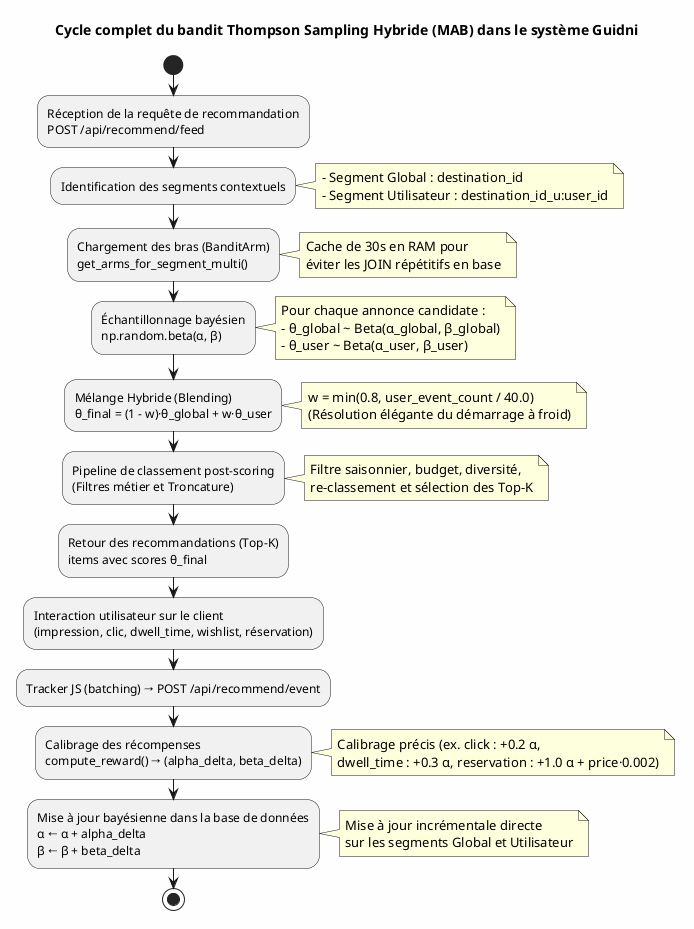
\includegraphics[width=0.85\textwidth]{diagrams/fig_02_ts_cycle.png}
    \caption{Cycle complet du bandit Thompson Sampling Hybride dans le système Guidni}
    \label{fig:ts_cycle}
\end{figure}

\subsection{Le modèle probabiliste Beta-Binomial}

Dans le cas d'interactions de type succès/échec (Bernoulli), la loi conjuguée naturelle est la distribution Beta. Pour chaque annonce (ou bras) $a$, le système modélise le taux d'engagement attendu $\theta(a) \in [0, 1]$ à l'aide d'une distribution Beta de paramètres de forme $\alpha$ et $\beta$~:

\begin{equation}
    f(\theta; \alpha, \beta) = \frac{\theta^{\alpha - 1} (1 - \theta)^{\beta - 1}}{\mathrm{B}(\alpha, \beta)}
\end{equation}

Les paramètres de la distribution sont mis à jour analytiquement après observation de l'engagement de l'utilisateur~:
\begin{itemize}
    \item \textbf{Succès} (clic, réservation) : $\alpha \leftarrow \alpha + \alpha_{\Delta}$
    \item \textbf{Échec / Pénalité} (impression sans clic, sortie rapide) : $\beta \leftarrow \beta + \beta_{\Delta}$
\end{itemize}

Cette approche bayésienne permet une gestion particulièrement robuste de l'incertitude : les nouvelles annonces
ayant peu d'expositions ont de très faibles valeurs d'hyperparamètres $\alpha$ et $\beta$ (par exemple, la valeur a priori par défaut $\alpha=1, \beta=1$). La variance de leur distribution est élevée, ce qui aplatit la courbe de probabilité et autorise temporairement des tirages de scores élevés (exploration). Dès que les données s'accumulent, la somme $(\alpha + \beta)$ augmente, la variance converge vers zéro, et la distribution se concentre étroitement autour de la vraie espérance bayésienne (exploitation pure).

\subsection{Segmentation de contexte et Calibrage des Récompenses}

Dans notre système Guidni, pour adapter les recommandations au contexte géographique et individuel de manière asynchrone et performante, le moteur Thompson Sampling introduit une double segmentation sémantique :

\begin{itemize}
    \item \textbf{Segment Global} : Représente la destination choisie par le visiteur (par exemple, \texttt{"djerba"}). Les statistiques collectives de performance de chaque annonce y sont stockées.
    \item \textbf{Segment Utilisateur} : Associe la destination et l'identifiant unique du voyageur (par exemple, \texttt{"djerba\_u:userId"}). Cela permet de modéliser des affinités individuelles uniques de façon isolée.
\end{itemize}

Les signaux comportementaux du tracker client sont traduits à travers un barème de calibrage précis, allant de la légère pénalisation passive d'impression ($\beta + 0.1$) au succès absolu de la réservation ($\alpha + 1.0$). De plus, pour favoriser la viabilité commerciale de la plateforme, le succès de réservation intègre un bonus financier direct proportionnel au prix de l'annonce~:
\begin{equation}
    \alpha_{\Delta}^{\text{reservation}} = 1.0 + 0.002 \times \text{prix}
\end{equation}
Cette formulation permet d'aligner l'optimisation mathématique du bandit avec le rendement économique de la place de marché Guidni.

\subsection{Résolution du Démarrage à Froid par Mélange Hybride}

Le problème de démarrage à froid (\textit{cold-start}) est résolu élégamment en combinant de façon linéaire les distributions globales et personnalisées lors de l'échantillonnage. Le score de pertinence final $\theta_{\text{final}}(a)$ est calculé par la formule de mélange hybride suivante~:

\begin{equation}
    \theta_{\text{final}}(a) = (1 - w) \times \theta_{\text{global}}(a) + w \times \theta_{\text{user}}(a)
\end{equation}

où $\theta_{\text{global}}(a) \sim \text{Beta}(\alpha_{\text{global}}, \beta_{\text{global}})$ et $\theta_{\text{user}}(a) \sim \text{Beta}(\alpha_{\text{user}}, \beta_{\text{user}})$, et $w$ représente le poids de personnalisation défini en fonction du nombre d'interactions historiques $N$ de l'utilisateur :

\begin{equation}
    w = \min\left(0.8, \frac{N}{40}\right)
\end{equation}

Ce mécanisme garantit une transition fluide de la recommandation de groupe (lorsque $w=0$) vers une affinité hautement personnalisée (lorsque $w$ grandit), tout en conservant une fraction de 20\% de poids collectif pour introduire de la nouveauté et éviter les phénomènes d'auto-enfermement.cteur $\phi$ de longueur
$9 \times 40 = 360$ qui capture les effets d'interaction --- par exemple, \og{}utilisateur
famille + tag pool\fg{} constitue une dimension unique du vecteur.

Un mécanisme de sécurité par hachage du vocabulaire garantit la cohérence entre le vocabulaire
et les matrices. Au démarrage, un hash SHA-256 du vocabulaire de tags trié est calculé par la
fonction \texttt{compute\_vocab\_hash()} et comparé au hash stocké dans la table
\texttt{SystemConfig}. Si les hash divergent, le système refuse de démarrer, empêchant une
corruption silencieuse de la matrice~$A$.

\begin{table}[H]
    \centering
    \caption{Les 9 composantes du vecteur utilisateur $x_{\text{user}}$}
    \label{tab:user_vector}
    \small
    \begin{tabular}{c l l c}
        \toprule
        \textbf{Idx} & \textbf{Caractéristique} & \textbf{Formule} &
        \textbf{Exemple} \\
        \midrule
        0 & sin(heure) & $\sin(2\pi \times h / 24)$ & $0.500$ \\
        1 & cos(heure) & $\cos(2\pi \times h / 24)$ & $-0.866$ \\
        2 & sin(mois) & $\sin(2\pi \times m / 12)$ & $-0.866$ \\
        3 & cos(mois) & $\cos(2\pi \times m / 12)$ & $-0.500$ \\
        4 & Profondeur défilement & $\text{clip}(\text{scroll}, 0, 1)$ & $0.70$ \\
        5 & Temps consultation & $\text{clip}(\log_e(1+\text{dwell})/\log_e(301), 0, 1)$ & $0.72$ \\
        6 & Affinité prix & $\text{avg\_price} / 2000$ & $0.075$ \\
        7 & Affinité tag max & $\max(\text{tag\_affinity})$ & $0.82$ \\
        8 & Type voyage & famille$=1.0$, couple$=0.67$, solo$=0.33$ & $1.0$ \\
        \bottomrule
    \end{tabular}
    \vspace{0.2cm}
    \footnotesize
    \begin{minipage}{10cm}
        \vspace{0.2cm}
        \footnotesize \textit{Exemple~: utilisateur famille, 10h du matin, mois d'août, 60s de consultation.}
    \end{minipage}
\end{table}


\subsection{Pipeline de classement post-scoring}

Le score brut échantillonné ne suffit pas seul à garantir une expérience utilisateur idéale. Plusieurs contraintes métier doivent être appliquées en post-traitement~: diversité des types d'annonces, adéquation budgétaire et géographique, et cohérence saisonnière. Le module de classement de Guidni applique un pipeline séquentiel d'étapes de filtrage et d'ajustement dans un ordre rigoureux autour de l'échantillonnage de Thompson Sampling.

Les étapes du pipeline sont les suivantes~:

\begin{enumerate}[leftmargin=2cm]
    \item \textbf{Identification du segment} : Détermination de la destination géographique courante et de l'identifiant utilisateur pour cibler les clés globales et utilisateur en base de données.
    \item \textbf{Récupération des candidats} : Extraction des bras éligibles depuis le cache en mémoire RAM (séparation des lectures pour garantir des temps de réponse sous 5\,ms).
    \item \textbf{Filtre saisonnier} : Retrait des annonces inadaptées à la saison touristique courante.
    \item \textbf{Filtre budgétaire} : Retrait des annonces dont le prix dépasse largement les contraintes ou le profil budgétaire estimé du voyageur.
    \item \textbf{Échantillonnage global} : Tirage probabiliste $\theta_{\text{global}}$ à partir de la loi $\text{Beta}(\alpha_{\text{global}}, \beta_{\text{global}})$.
    \item \textbf{Échantillonnage utilisateur} : Tirage probabiliste $\theta_{\text{user}}$ à partir de la loi $\text{Beta}(\alpha_{\text{user}}, \beta_{\text{user}})$ si l'historique utilisateur existe.
    \item \textbf{Mélange hybride} : Application de la formule de pondération $\theta_{\text{final}} = (1 - w)\theta_{\text{global}} + w\theta_{\text{user}}$ pour résoudre le démarrage à froid.
    \item \textbf{Filtre de diversité} : Limiter la redondance d'une même catégorie (par exemple, éviter d'afficher 8 hébergements consécutifs, garantissant un flux diversifié d'activités, de restaurants et d'attractions).
    \item \textbf{Tri par marge commerciale} : En cas d'écart de score négligeable, ordonnancement par taux de commission pour maximiser le rendement financier de la plateforme.
    \item \textbf{Troncature} : Sélection des \texttt{top\_k} meilleurs éléments (par défaut 8) avant envoi de la réponse JSON au client.
\end{enumerate}



% ────────────────────────────────────────────────────────────────
\section{Travaux connexes et comparaison}
% ────────────────────────────────────────────────────────────────

Les approches classiques de bandits contextuels linéaires ont été introduites dans le contexte de la
recommandation d'articles de presse sur le portail Yahoo! Today~\cite{li2010linucb}. Ces travaux ont démontré que
les bandits linéaires surpassent les méthodes classiques lorsque
le contenu évolue rapidement.
Bouneffouf et al.~\cite{bouneffouf2014context} ont étendu ces approches aux recommandations
mobiles avec des bandits hybrides intégrant des signaux contextuels. Le \textit{Thompson Sampling} constitue une alternative
bayésienne particulièrement robuste. C'est cette approche qui a été retenue et optimisée dans ce projet de fin d'études sous sa forme Hybride (Beta-Binomiale), pour sa scalabilité exceptionnelle en $O(1)$, sa haute interprétabilité et sa capacité naturelle à équilibrer exploration et exploitation sans hyperparamètres arbitraires à calibrer.


Booking.com a développé un système de classement hybride sophistiqué, intégrant des signaux
en temps réel et une infrastructure de tests A/B à grande échelle~\cite{bernardi2019booking}.
Cependant, ce système est entièrement fermé et non reproductible, conçu pour un volume de
trafic de plusieurs ordres de grandeur supérieur à celui d'une place de marché touristique
locale. Les techniques employées (réseaux de neurones profonds, infrastructure de feature store
distribuée) ne sont pas adaptées au contexte d'un projet académique avec des contraintes de
ressources limitées.

Dans le domaine de la planification de voyage automatisée, Lim et al.~\cite{lim2018personalized}
et Jiang et al.~\cite{jiang2019trip} proposent des approches par optimisation combinatoire
sur des graphes de points d'intérêt. Ces travaux modélisent la planification comme un problème
d'optimisation sous contraintes (temps, budget, distance) mais n'intègrent pas d'interaction
conversationnelle, de données météorologiques en temps réel, ni d'apprentissage en ligne à
partir du comportement utilisateur.

\begin{table}[H]
    \centering
    \caption{Comparaison avec les systèmes existants}
    \label{tab:comparison}
    \small
    \begin{tabular}{p{3cm} c c c c c}
        \toprule
        \textbf{Système} & \textbf{Planif.} & \textbf{Reco. TR} &
        \textbf{Multilingue} & \textbf{Apprent. OL}  \\
        \midrule
        Guidni (ce projet) & \checkmark & \checkmark & \checkmark & \checkmark  \\
        TripAdvisor & $\times$ & $\times$ & \checkmark & $\times$  \\
        Booking.com & $\times$ & \checkmark & \checkmark & \checkmark \\
        ChatGPT (sans outils) & Partiel & $\times$ & \checkmark & $\times$  \\
        \bottomrule
    \end{tabular}
    \vspace{0.2cm}
    \footnotesize
    \begin{minipage}{10cm}
        \vspace{0.2cm}
        \textit{Planif.~= planification multi-jours, Reco. TR~= recommandation temps réel,
        Apprent. OL~= apprentissage en ligne.}
    \end{minipage}
\end{table}


% ────────────────────────────────────────────────────────────────
\section{Choix technologiques et justification}
% ────────────────────────────────────────────────────────────────

\textbf{FastAPI} a été préféré à Django et Flask pour sa nature nativement asynchrone, sa
génération automatique de documentation OpenAPI, sa validation des données par Pydantic, et ses
performances supérieures pour les tâches d'entrée-sortie intensives typiques des applications IA.
L'agent LLM effectue de multiples appels réseau concurrents (LLM, base de données, APIs
météo, géocodage), rendant l'asynchronicité essentielle.

\textbf{LangGraph} a été choisi plutôt que LangChain Expression Language (LCEL) ou CrewAI pour
son état explicitement typé qui facilite le débogage, son graphe orienté qui permet des boucles
de validation impossibles avec des chaînes linéaires, son support natif du streaming, et sa
flexibilité pour définir des fonctions de routage conditionnel complexes.

\textbf{LlamaIndex} a été préféré à FAISS ou Chroma pour sa gestion intégrée du magasin de
documents (\textit{document store}), son filtrage par métadonnées nativement supporté, sa
persistance automatique sur la base de données Qdrant, et sa capacité à gérer les mises à jour 
unitaires (insertion/suppression ciblée), s'intégrant parfaitement avec les tâches asynchrones 
déclenchées par nos triggers SQL pour la réindexation incrémentale.

\textbf{BAAI/bge-m3} a été sélectionné plutôt que OpenAI \texttt{text-embedding-3} car il est
gratuit, s'exécute localement (aucune donnée transmise à des tiers), supporte nativement le
français, l'anglais et l'arabe, et n'introduit aucune dépendance réseau pour la recherche
sémantique.

\textbf{Thompson Sampling Hybride} a été préféré aux approches déterministes classiques et aux bandits neuronaux pour quatre raisons fondamentales : (1) sa complexité algorithmique unitaire stricte en $O(1)$ par bras contre le coût quadratique ou cubique des calculs matriciels des modèles de bandits linéaires déterministes, (2) sa lisibilité théorique optimale où les paramètres $\alpha$ (succès) et $\beta$ (échecs) sont directement exploitables en base de données, (3) sa gestion naturelle du dilemme exploration-exploitation via l'échantillonnage probabiliste bayésien, et (4) son élégante formule de mélange hybride qui résout nativement le problème de démarrage à froid pour les nouveaux utilisateurs.

\textbf{SQLAlchemy} a été retenu comme ORM principal pour gérer les interactions standards 
avec la base de données relationnelle en raison de sa robustesse. Toutefois, la capture 
des modifications (insertions, mises à jour et suppressions) nécessaires à la réindexation 
a été sciemment extraite de la couche applicative et déléguée à des \textbf{triggers} 
nativement intégrés au SGBD. Cette séparation des préoccupations décharge SQLAlchemy 
de la logique de synchronisation, offrant ainsi un couplage faible et garantissant que 
toute modification des données, même externe à l'application, soit automatiquement captée.

Le \textbf{tracker JavaScript} a été développé sans dépendance externe (ni Google
Analytics, ni Segment) pour garantir un contrôle total sur les données collectées, éliminer
les cookies tiers, assurer la conformité RGPD, et offrir un poids de chargement minimal.


% ────────────────────────────────────────────────────────────────
\section*{Conclusion du chapitre}
\addcontentsline{toc}{section}{Conclusion du chapitre}
Ce chapitre a établi les fondements théoriques nécessaires à la compréhension du système Guidni.
Les agents LLM et le patron ReAct ont été présentés comme base de l'architecture agentique, le
framework LangGraph a été justifié comme choix de machine à états pour sa debuggabilité et ses
boucles de validation, et l'abstraction multi-fournisseurs LLM a été exposée pour sa flexibilité.
Le pipeline RAG avec le modèle d'embedding multilingue BAAI/bge-m3 et la réindexation automatique
pilotée par des \textbf{triggers} de base de données ont été décrits comme mécanisme de grounding 
factuel. Les systèmes de recommandation ont été comparés selon quatre axes, établissant la supériorité 
de l'apprentissage en ligne par bandits bayésiens pour le cas d'usage touristique. L'algorithme 
Thompson Sampling Hybride a été formalisé mathématiquement, la modélisation conjuguée Beta-Binomiale
a été détaillée avec son barème de calibrage comportemental et son mélange d'échantillonnage global-personnalisé, et le pipeline 
de classement post-scoring en \textbf{dix} étapes a été décrit.

Le chapitre suivant traduira ces fondements théoriques en exigences concrètes, modèles UML et
conceptions architecturales détaillées pour les deux sous-systèmes du projet Guidni.